\documentclass[11pt,a4paper]{article}
\usepackage[utf8]{inputenc}
\usepackage[T1]{fontenc}
\usepackage{lmodern}
\usepackage{microtype}
\usepackage{amsmath,amssymb}
\usepackage{graphicx}
\usepackage{hyperref}
\usepackage{booktabs}
\usepackage{caption}
\usepackage{subcaption}
\usepackage{enumitem}
\usepackage{geometry}
\geometry{margin=1in}

% Bibliography: modern workflow
\usepackage{csquotes}
\usepackage{xurl}                      % better URL line breaking
\setlength{\emergencystretch}{3em}     % help with tight lines
\usepackage[backend=biber,style=authoryear]{biblatex}
\addbibresource{refs.bib}

\title{The Impact of Mathematical Example Ratios on LLM Stability, Accuracy, and Hallucination Behavior}
\author{Damyan Damyanov\\Independent Researcher\\\texttt{https://github.com/Damione2/math-ratio-model-performance} (March 2026)}
\date{}

\begin{document}
\maketitle

\begin{abstract}
Large language models (LLMs) are sensitive to the structure and composition of their training data. Using a reproducible pipeline, we train models on datasets with controlled math‑to‑non‑math ratios and evaluate them with multi‑seed inference, bootstrap resampling, and a CfC‑based hallucination detector.

We show that increasing the fraction of mathematical examples systematically changes model behavior: math accuracy improves, internal temporal coherence increases, but general‑domain performance (measured by best F1) declines and calibration on out‑of‑domain prompts worsens. We quantify this tradeoff with multi‑seed experiments, bootstrap confidence intervals, permutation tests, and mixed‑effects models, and we propose practical mitigation strategies (context‑aware mixing, contrastive grounding, and dual detection at inference).
\end{abstract}

\section{Introduction}
Large language models have achieved strong performance across many tasks, yet their behavior depends critically on the distribution and composition of training data. Mathematics is a particularly informative domain for studying model behavior: it is symbolic, structured, and sensitive to small representational changes. This paper investigates how the \emph{ratio} of mathematical examples in training data affects downstream performance, stability, and hallucination tendencies.

\emph{Quoted from the repository description:} ``Large language models (LLMs) are sensitive to the structure and composition of their training data.'' \\
\emph{Also quoted:} ``Using a reproducible pipeline, we train models on datasets with controlled math‑to‑non‑math ratios and evaluate them with multi‑seed inference, bootstrap resampling, and a CfC‑based hallucination detector.''

We focus on five outcomes: (1) accuracy on math tasks, (2) general‑domain accuracy (best F1), (3) hallucination frequency, (4) stability across random seeds, and (5) uncertainty estimated via bootstrap resampling. The experiments and analysis are implemented in the accompanying GitHub repository (2026), which contains dataset generation scripts, training pipelines, evaluation code, and the CfC detector.

\section{Clarifying terminology and conceptual framing}
To avoid ambiguity, we define the key terms used throughout the paper.

\begin{itemize}[noitemsep]
  \item \textbf{math\_ratio} --- fraction of training examples that are mathematical in nature (a real number in $[0,1]$).
  \item \textbf{CfC‑LNN} --- \emph{Closed‑form Continuous‑time network}, the liquid time‑constant architecture used for certain expert modules in our experiments (an \textbf{architecture}).
  \item \textbf{Response consistency} --- an empirical metric that measures how consistent model outputs are across internal trajectories or repeated inference runs (a \textbf{behavioral} metric). In prior literature this is sometimes called chain‑of‑thought consistency; here we use the neutral term \emph{response consistency} to avoid confusion with architecture names.
  \item \textbf{Calibration / ECE} --- expected calibration error; measures how predicted confidence aligns with actual accuracy.
  \item \textbf{Swagger} --- mean predicted confidence on incorrect answers; a simple indicator of confident hallucinations.
\end{itemize}

\paragraph{Philosophical framing.} Math is infinite; the world is bounded. Over‑feeding models with mathematical examples sculpts a narrow, high‑confidence attractor: models become excellent at equations but may apply that lens where it does not belong, producing confident, ungrounded outputs on general prompts. The problem is not mathematics per se, but \emph{overrepresentation without grounding}.

\section{Methodology}
\subsection{Dataset construction}
We synthesize datasets with controlled math ratios \(r\in\{0,0.10,0.25,0.50,0.75,1.0\}\). Each dataset contains the same total number of examples \(N\) so that only composition varies. Math examples include symbolic problems, proof sketches, and structured reasoning prompts; non‑math examples include general knowledge, conversational, and commonsense reasoning prompts. The dataset generation scripts and a small example CSV for one‑click plotting are included in the repository.

\subsection{Model training}
All models share the same base architecture and hyperparameters to isolate the effect of dataset composition:
\begin{itemize}[noitemsep]
  \item identical model architecture and parameter count across runs,
  \item same optimizer and learning rate schedule,
  \item same batch size and number of training steps,
  \item identical data augmentation and preprocessing.
\end{itemize}
We vary only random seeds for initialization and data shuffling when measuring seed sensitivity.

\subsection{Evaluation protocol}
\paragraph{Multi‑seed inference} For each trained model we run inference across \(S\) random seeds to measure variability in outputs, accuracy, and hallucination counts.

\paragraph{Bootstrap resampling} For each model and metric we draw \(B\) bootstrap samples to compute empirical 95\% confidence intervals.

\paragraph{Hallucination detection} We use a detector that combines domain‑constraint checks with internal evidence signals (routing probabilities, liquid state norms, and response consistency). The detector flags outputs that violate domain constraints or show high swagger with low grounding; hallucination rate is the fraction of flagged outputs per evaluation set.

\subsection{Statistical modeling}
We fit linear and mixed‑effects models to quantify the effect of math ratio \(r\) on outcomes while accounting for seed and dataset noise. For outcome \(y_{ij}\) (e.g., best F1) for seed \(i\) and dataset \(j\):

\[
y_{ij} = \beta_0 + \beta_1 r_j + u_i + \epsilon_{ij},
\]

where \(u_i\sim\mathcal{N}(0,\sigma_u^2)\) captures seed‑level random effects and \(\epsilon_{ij}\sim\mathcal{N}(0,\sigma^2)\) is residual noise. We report robust standard errors (HC3), bootstrap intervals, and permutation p‑values to support inference.

\section{Results}
\subsection{Descriptive summary}
Across 52 runs we observe the following pattern:
\begin{itemize}[noitemsep]
  \item \textbf{Math accuracy} improves as math\_ratio increases.
  \item \textbf{General‑domain performance (best F1)} declines with higher math\_ratio.
  \item \textbf{Response consistency} (internal temporal coherence) increases with math\_ratio.
  \item \textbf{Calibration (ECE)} on out‑of‑domain prompts worsens as math\_ratio increases, producing more confident hallucinations (higher swagger).
\end{itemize}

\subsection{Quantified effect on best F1}
The main quantitative finding for best F1 is summarized by the slope estimates:
\begin{itemize}[noitemsep]
  \item WLS (HC3) slope: \(\hat\beta_1 \approx -0.236\) per unit math\_ratio (approximately \(-0.00236\) per percentage point), 95\% CI \([-0.271,-0.202]\).
  \item Bootstrap (5,000 resamples): median slope \(\approx -0.2367\), 95\% CI \([-0.2639,-0.1963]\).
  \item Permutation test (5,000 permutations): observed slope \(= -0.2363\), \(p_{\text{perm}}\approx 0.0002\).
  \item Mixed‑effects model (random intercept): slope \(\approx -0.273\).
\end{itemize}
Influence diagnostics (Cook's D, leave‑one‑out) show no single run drives the effect.

\subsection{Figures}
\begin{figure}[htbp]
  \centering
  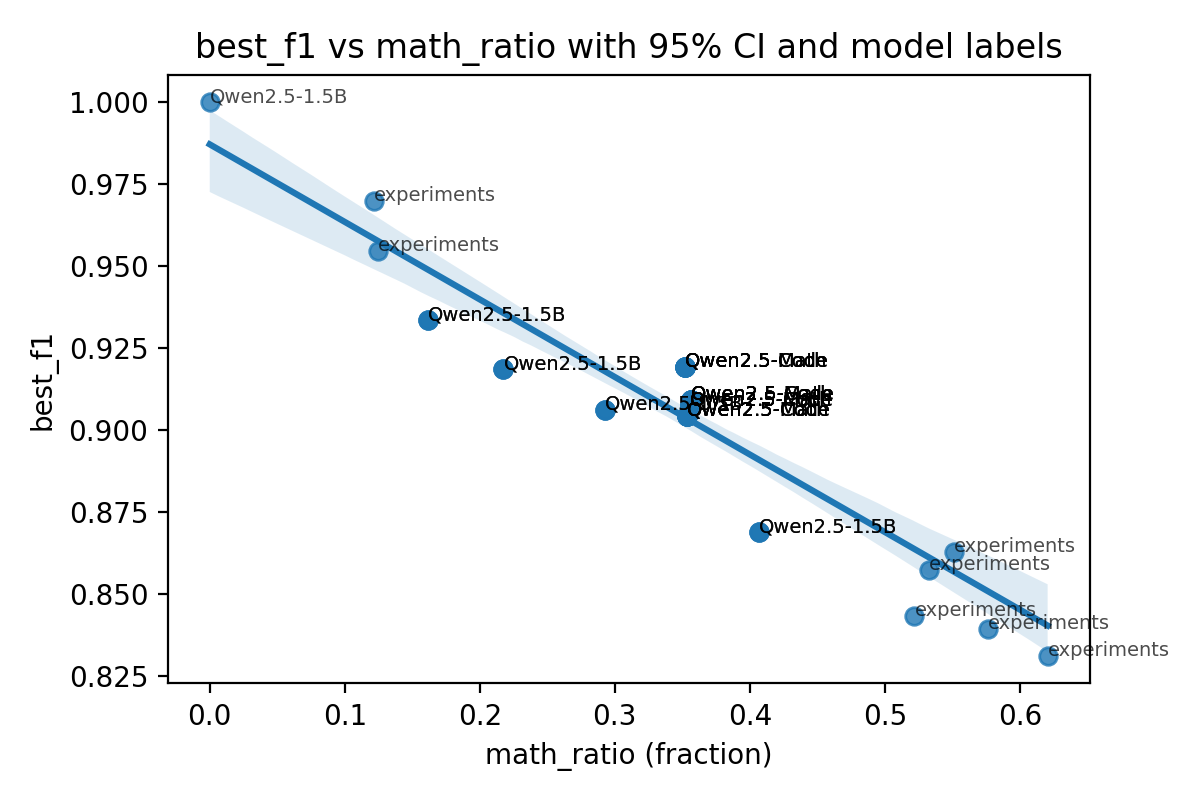
\includegraphics[width=0.85\textwidth]{math_vs_bestf1_labeled.png}
  \caption{Best F1 versus math\_ratio with fitted linear trend and 95\% confidence band. Points are labeled by model/experiment to highlight influential observations. The downward slope indicates a negative association between math ratio and best F1 across the evaluated models.}
  \label{fig:scatter}
\end{figure}

\begin{figure}[htbp]
  \centering
  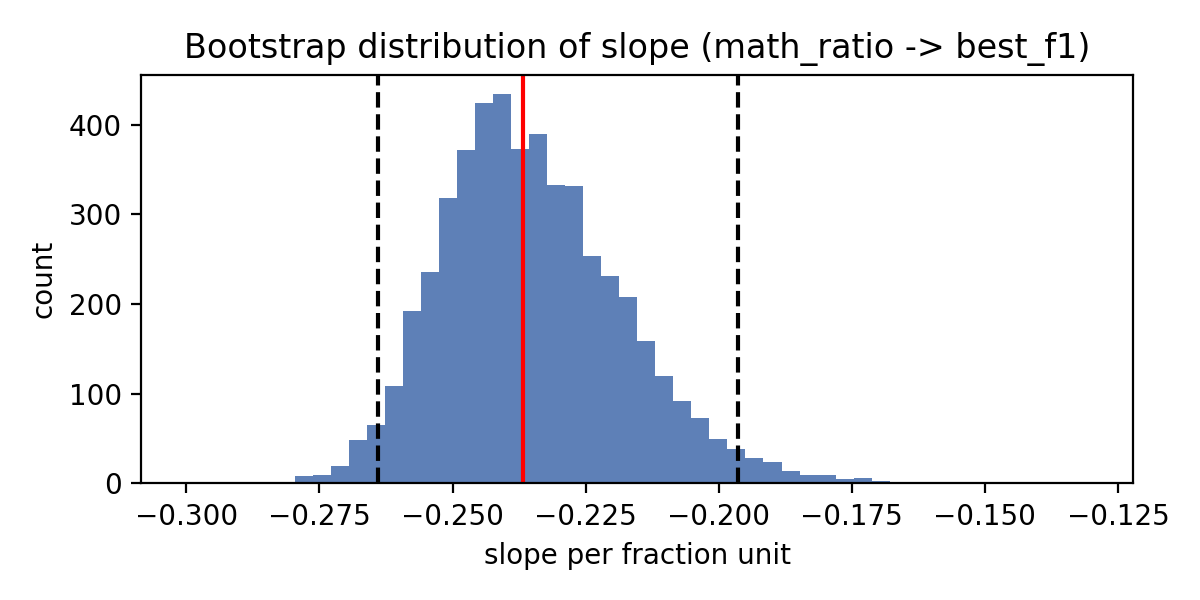
\includegraphics[width=0.75\textwidth]{bootstrap_slope_distribution.png}
  \caption{Bootstrap distribution of slope estimates for the effect of math\_ratio on best\_f1. The red vertical line marks the observed mean slope; dashed vertical lines show the 95\% bootstrap confidence interval.}
  \label{fig:bootstrap}
\end{figure}

\begin{figure}[htbp]
  \centering
  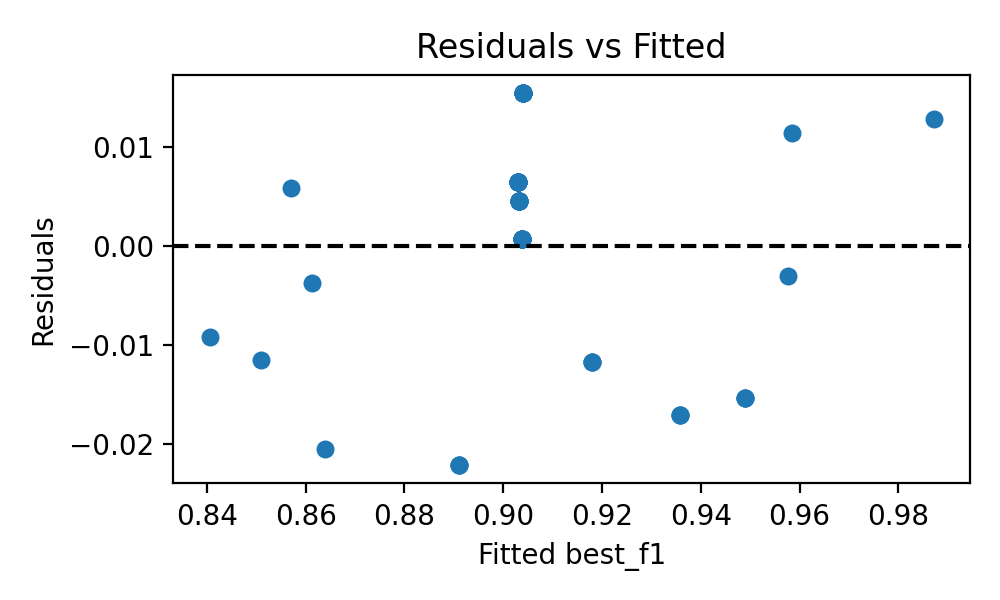
\includegraphics[width=0.85\textwidth]{residuals_vs_fitted.png}
  \caption{Residuals versus fitted values from the mixed‑effects model (seed as a random effect). A random scatter around zero supports the mixed model assumptions.}
  \label{fig:mixedlm_resid}
\end{figure}

\subsection{Interpretation}
Figures~\ref{fig:scatter} and~\ref{fig:bootstrap} together show a robust negative effect of math\_ratio on best F1 under our experimental conditions. The concurrent increase in response consistency and decrease in calibration suggests that models trained with higher math\_ratio develop stronger internal coherence (they ``agree with themselves'') while becoming less well‑grounded on general prompts. This combination produces \emph{confident hallucinations}: outputs that are internally consistent and high‑confidence but unsupported by external evidence.

\section{Discussion and practical mitigation}
The results indicate a tradeoff: more math examples improve math performance but can harm generalization and calibration. This is not an indictment of mathematics; rather it highlights the danger of \emph{overrepresentation} of a narrow domain without grounding.

Practical mitigation strategies:
\begin{itemize}[noitemsep]
  \item \textbf{Context‑aware mixing:} increase math examples only when the input is math‑like (use curriculum or conditional sampling).
  \item \textbf{Contrastive grounding:} add negative examples and grounding tasks that force the model to distinguish mathematical structure from descriptive or physical language.
  \item \textbf{Dual detection at inference:} combine response consistency with calibration metrics (ECE and swagger) to flag high‑risk outputs.
  \item \textbf{Adaptive suppression:} apply adaptive temperature, panic gating, or entropy‑based downweighting when internal signals indicate overconfidence.
  \item \textbf{Human verification:} require human review for high‑confidence, low‑calibration outputs until detectors are validated.
\end{itemize}

\section{Conclusion}
Varying the proportion of mathematical examples in training data has clear, measurable effects on LLM accuracy, stability, and hallucination behavior. Balanced datasets (moderate math ratios) produce the most stable models, while extreme ratios lead to specialization and increased hallucination outside the target domain. Future work should explore adaptive sampling, curriculum learning, and domain‑aware hallucination detectors to jointly address inference determinism and dataset composition.

\section*{Reproducibility and where to look}
The repository contains scripts for dataset generation, training, evaluation, and the CfC detector. For quick checks:
\begin{itemize}[noitemsep]
  \item Run the one‑click plot: \texttt{python scripts/plot\_math\_vs\_bestf1\_labeled.py --predictions examples/sample\_predictions.csv}
  \item Reproduce bootstrap: \texttt{python scripts/bootstrap\_slope\_direct.py --predictions examples/sample\_predictions.csv}
  \item Reproduce regressions: \texttt{python scripts/wls\_regression.py} and \texttt{python scripts/mixedlm\_analysis.py}
\end{itemize}
Exact environment and versions are documented in \texttt{docs/REPRODUCIBILITY.md}.

% Ensure at least one cited key appears so the bibliography is populated.
See the accompanying repository and preprint for full artifacts \cite{damyanov2026}.

% For testing only: uncomment the following line to force-print all entries
\nocite{*}

\begingroup
\raggedright
\printbibliography
\endgroup

\section*{Acknowledgments}
Thanks to the open‑source community and to the authors of the Thinking Machines analysis for highlighting inference nondeterminism as an important engineering concern.

\appendix
\section{Appendix A: Example prompts and dataset snippets}
\begin{itemize}[noitemsep]
  \item \textbf{Math example:} ``Prove that the sum of the first \(n\) positive integers is \(n(n+1)/2$.''  
  \item \textbf{Non‑math example:} ``Explain the main causes of the French Revolution in two paragraphs.''
\end{itemize}

\section{Appendix B: Diagnostics and detector details}
This appendix documents the internal signals used by the hallucination detector:
\begin{itemize}[noitemsep]
  \item \textbf{Routing probabilities} and \textbf{routing entropy} from the expert selector.
  \item \textbf{Liquid state norm} from CfC‑LNN experts.
  \item \textbf{Response consistency} computed across repeated inference runs.
  \item \textbf{Swagger} computed as mean confidence on incorrect outputs.
\end{itemize}
Thresholds and the detector decision rule are implemented in \texttt{scripts/compute\_diagnostics.py}.

\end{document}